\section{On-going Work}
\label{sec:ongoing_work}

While the Nova revision we presented in the previous
sections is a promising proof-of-concept toward widely distributed OpenStack
infrastructures, there are remaining challenges that need to be tackle.

%First, it is critical to study whether similar changes can be achieved on other components.
%Second, the notion of locality does not exist in our current implementation.
%That is, any request can be served by any controller available, leading to the creation of a VM anywhere in the infrastructure.

In  this section,  we present  two on-going  actions that  aim at  deepening the
relevance of our approach. First,  we show that existing seggregation mechanisms
provided by OpenStack are not satisfactory  when it comes to reducing inter-site
communications.
%  in  order to  improve  networking  efficiency of  a  multi-site OpenStack  deployment.
In  response,  two actions  could be  made:  on one  hand
introducing  networking  locality  in  the   shared  databases  and  the  shared
messaging, on the other hand distributing remaining services of OpenStack.

%While the achievement of such
%changes are under heavy development, we believe that our approach is promising
%enough to favor the adoption of the distributed cloud model supervised by a
%single system.

Second, we discuss the preliminary study we  made on the Glance image service to
investigate whether it is possible to apply similar modifications to the ones we
performed on Nova. Such a validation is  critical as Glance is a key element for
operating a production-ready IaaS infrastructure.

These two actions clearly demonstrate that our approach is promising
enough to favor the adoption of the distributed cloud model supervised by a
single system.

\subsection{Locality Challenges / $\mu$cro DCs Segregation}

%% Even if this article has demonstrated that the relational database used by Nova
%% could be replaced by a non relational key/value store, a more advanced
%% validation of this change is required and the question of which metrics to use
%% remains. On one hand, a larger deployment involving more geographical sites
%% would be more demonstrative, on the other hand the changes we introduced have
%% been have been motivated by more than overall scalabity, but also fault
%% tolerance and reduction of response times when processing API requests.

%% \subsection{Distributing the remaining services of OpenStack}

%% As introduced in section \ref{leveraging-openstack}, the other services
%% composing OpenStack are historically leveraging a relational database to store
%% their inner-states. As done with Nova, this relational database may be replaced
%% by a key/value data-store. Among the remaining services, the next candidate is
%% the image service Glance: as its images are already stored in fully distributed
%% cloud storage software (SWIFT), the next step to reach a fully distributed
%% functionning with Glance is to apply the same strategy that we did with Nova. On
%% the other  hand, the situation may be different with some other services:
%% Neutron works  with drivers that may be intented to work in a distributed way.
%% In such  situation alternatives have to be found.

%% \subsection{Locality aware objects in OpenStack}

%% Having a wan-wide infrastructure can be source of networking overheads: some
%% objects manipulated by OpenStack are subject to be manipulated by any service of
%% the deployed controllers, and by extension should be visible to any of the
%% controllers. On the other hand, some objects may benefit from a restrained
%% visibility: if a user has build an OpenStack project (tenant) that is based on
%% few sites, appart from data-replication there is no need for storing objects
%% related to this project on external sites. Restraining the storage of such
%% objects according to visibility rules would enable to save network bandwidth and
%% to settle policies for applications such as privacy and efficient data-
%% replication.

Deploying  a massively  multi-site  Cloud Computing  infrastructure operated  by
OpenStack   is  challenging   as  communication   between  nodes   of  different
geographical clusters can be subject to  an important network latency, which can
be a source of disturbances for OpenStack. Experimental results presented in the
Table~\ref{tab:orgtable2}  of  Section~\ref{sec:multisite_exps}  clearly  showed
that an  OpenStack distributed  on top  of our  Rome+REDIS solution  can already
operate over an  ISP network with a high inter-site  latency (50~ms). While this
result is  positive and can indicate  that such a configuration  is appropriated
for operating  a distributed  CC infrastructure  involving tens  of geographical
site,  it   is  important   to  understand  the   nature  of   network  traffic.
Table~\ref{tab:experiments-host-aggregates-network}  shows   the  total  traffic
\textit{vs.} the  traffic between  the remote  sites using  a 4  sites OpenStack
leveraging  our Rome+REDIS  proposal and  with the  host-aggregate feature.  The
first  line clearly  shows that  even with  the host-aggregate  feature enabled,
there is a dramatic amount of communications (87.7\%) made between nodes located
in distinct geographical sites.

\begin{table}[htb]
\vspace{-0.5cm}
\caption{\label{tab:experiments-host-aggregates-network}
  Quantity of data exchanged over network (in MBytes)}
\centering
\begin{tabular}{lrrr}
 & Total  & Inter-site &  Proportion \\
\hline
%without host-aggregates & 4484 & 4171 & 93.0\% \\
%with host-aggregates & 5326 & 4672 & 87.7\% \\
4 clusters  & 5326 & 4672 & 87.7\% \\
\end{tabular}
\end{table}

%% The  first  approach that  came  to  mind to  reduce  the  amount of  inter-site
%% communication is  to seggregate nodes  composing the infrastructure  by grouping
%% nodes of a same site or from close  sites. We tested such a strategy by grouping
%% each  node of  a same  site in  a same  host-aggregates/availability-zone, which
%% enables to provide a finer control on the scheduling of a VM. The second line of
%% Table~\ref{tab:experiments-host-aggregates-network} shows  that despite  a minor
%% reduction of the proportion of inter-sites  communications, it remains at a very
%% high level (87.7\%).

A quarter of these inter-site communications are caused by the isolation of Nova
from other OpenStack services (\ie Keystone and Glance) which were deployed on a
dedicated master node in our experiments. Indeed, operations like serving VM
images were naturally a source of artificial inter-site communications. This
situation clearly advocates in favor of massively distributing the remaining
services, as we did with Nova. Finally, as instances of OpenStack services
collaborate via a shared messaging bus and via a shared database, unless these
two elements will be able to avoid the broadcasting of information by taking
advantage of network locality, the level of inter-site communication will remain
large. We are investigating two directions. First, we are studying whether the
use of a P2P bus such as ZeroMQ\cite{zeromq:2013} can reduce such a network overhead and second
whether the service catalog of Keystone can become locality-aware in order to ``hide'' redundant services that are located remotely.


\subsection{Revising Glance: The OpenStack Image Manager}
Similarly to the Nova component (see Section \ref{subsec:mysql-to-redis}), only
the inner states of Glance are stored in a MySQL DB, the VM images are already
stored in a fully distributed way (leveraging either SWIFT or Ceph/Rados
solution \cite{weil2006ceph}). Therefore, our preliminary study aimed at
determining whether it was possible or not to reuse the ROME library to switch
between the SQL and NoSQL backends. As depicted by Figure \ref{fig:glance_dbs},
the Glance code from the software engineering point of view is rather close to
the Nova one. As a consequence, replacing the MySQL DB by a KVS system did not
lead to specific issues. We underline that the replacement of MySQL with REDIS
was even more straightforward than for Nova as Glance enables the configuration
of specific API for accessing persistent data (\texttt{data\_api} in the Glance
configuration file). We are currently validating that each request is correctly
handled by Rome. Preliminary performance experiments are planned for the
beginning of 2016.

%API to use for accessing data. Default value points to sqlalchemy
%# package, it is also possible to use: glance.db.registry.api
%# data_api = glance.db.sqlalchemy.api

\begin{figure}[htbp]
%\vspace*{-0.3cm} 
        \centering
        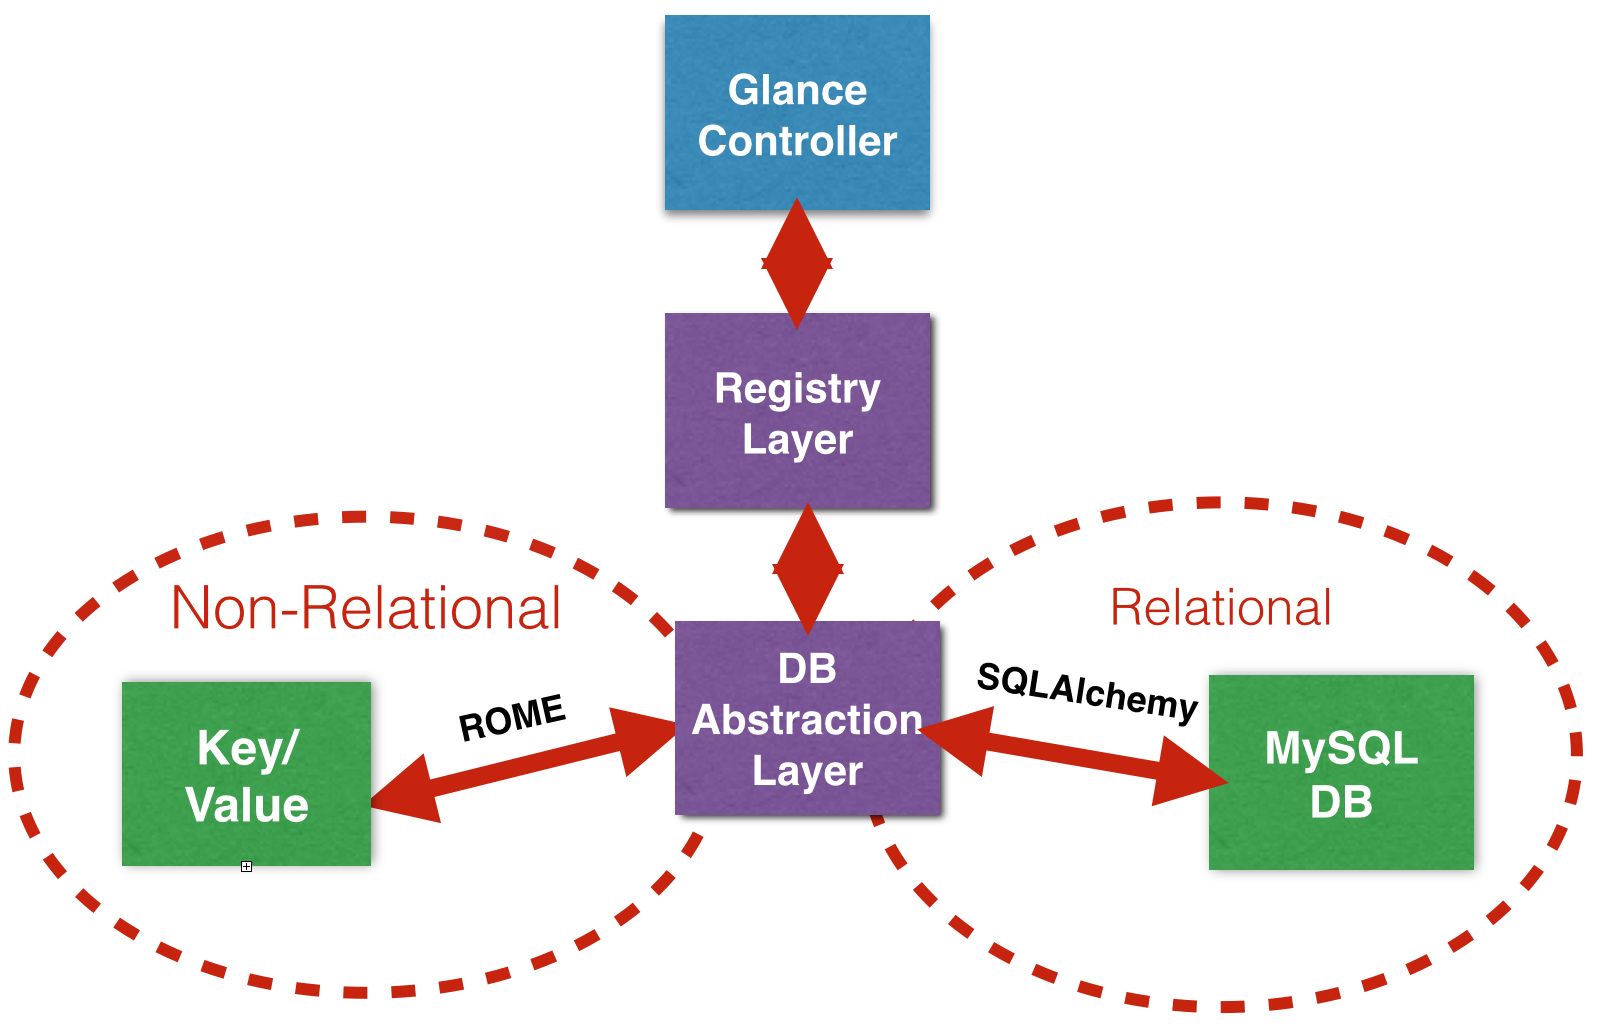
\includegraphics[width=8.5cm]{figures/rome_glance.png}
%\vspace*{-0.8cm}
        \caption{Glance - Software Architecture and DB dependencies.}
        \label{fig:glance_dbs}
%\vspace*{-.3cm}
\end{figure}
